\section{Spring support in IDE}

\begin{frame}
\frametitle{Spring support in IDE is a +}

\begin{itemize}
 \item e.g. code completion in SpringSource Tool Suite
\end{itemize}

\begin{figure}
\begin{center}
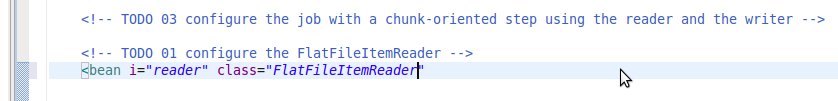
\includegraphics[width=10cm]{figures/before-cc.png}
\end{center}
\end{figure}

\begin{center}
\begin{picture}(0,0)
\put(0,15){\vector(0,-1){15}} 
\end{picture}
\end{center}

\begin{figure}
\begin{center}
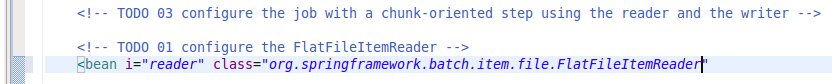
\includegraphics[width=10cm]{figures/after-cc.png}
\title{Code completion in SpringSource Tool Suite}
\end{center}
\end{figure}
 
\end{frame}

\begin{frame}[fragile]
 \frametitle{Shortened package names}
 \begin{itemize}
  \item{Be careful, a package name can sometimes be shortened}
 \end{itemize}
 \begin{xmlcode}
<bean class="c.z.workshop.springbatch.HelloWorldTasklet" />
 \end{xmlcode}
 \begin{itemize}
  \item{Type the name of the class, code completion will do the rest...}
 \end{itemize}
 \begin{xmlcode}
<bean class="com.zenika.workshop.springbatch.HelloWorldTasklet" />
 \end{xmlcode}
\end{frame}

